\section{Implementation, development methodologies}

mGov is meant to be used as a starter kit for building a custom governmental site. But before starting working with Drupal, you need to understand it. Therefore will continue with a guide that will give you an overview of Drupal, helping you to determine if drupal is a good fit for this project.

\subsection{Meeting Drupal}

To clarify the difference between Drupal and other CMSs, consider the example of a news site. You want to be able to post news articles on the site, and you want the homepage to have a section featuring the five most recent ones. Next, you decide that you want to add a blog section, and put a list of links to the five most recent blog entries on the homepage as well.

If you were using an ordinary CMS, first you would install a plugin that handled news articles and could put short blurbs on the homepage. Next, you would install a plugin that would track the latest blog posts and put a list of those on the homepage. Each plugin would only be responsible for tracking and managing a particular kind of content, and each would remain relatively isolated from the others.

But, what happens when you have that brilliant, middle-of-the-night idea to blend these two functions by showing a list of blog posts about the latest news items, ordered according to contributor activity? If you’re using a “toy truck” CMS, you may be out of luck. Or, you may need to hire a developer to write a custom plugin from scratch. But through the power of the Drupal way, the way of manageable abstraction, you can accomplish this task quickly and easily. Since Drupal's modules do things in a standard way and interface with a common underlying system, building all sorts of clever, customized features is just a matter of snapping parts together. In this example, you could just use Views.

Of course, this flexibility comes at a certain cost. While a toy truck is instantly understandable and ready to use without much thought, a modular vehicle construction kit will, by nature, require you to read the instruction manual first. The building blocks are available, but you'll need to learn how they fit together before you can take a paper prototype and turn it into a full-featured website.

Drupal core, and the thousands of contributed modules that build on it, requires an initial investment to learn, but mastering the Drupal way is immensely rewarding; the passionate community is a testament to Drupal's power to liberate site builders from the simplicity/flexibility dilemma. Once you've tried Drupal, you'll likely leave your toy truck and boat in the closet to gather dust.

\subsubsection{How Drupal works?}

People often think of a website as a collection of static pages, perhaps with some functions like a blog or a news engine thrown in to round it out. When they go to manage their site, they are thinking in terms of a tree-like hierarchy of pages that they will edit.

Drupal, however, treats most content types as variations on the same concept: a node. Static pages, blog posts, and news items are all stored in the same way, and the site's navigation structure is designed separately by editing menus, views lists of content, and blocks side content which often have links to different site sections.

It’s a lot like the separation you find in standards-compliant page coding—XHTML provides the meaningful structure of the information, while CSS arranges it for presentation. In Drupal, nodes hold the structured information pertaining to a blog post such as title, content, author, date or a news item, while the menu system, as well as taxonomy tagging of content and views, creates an information architecture. Finally, the theme system, along with display modules like Panels, controls how all this looks to site visitors.

Since these layers are kept separate, you can provide a completely different navigation and presentation of your content to different users based on their specific needs and roles. Pages can be grouped differently, prioritized in a different order, and various functions and content can be shown or hidden as needed.

\subsubsection{Nodes}

We don't talk about nodes every day, but since they are at the heart of Drupal's design, they deserve further investigation. Essentially, a node is a set of related bits of information. When you create a new blog post, you are not only defining its body text, but also its title, content, author link, creation date, taxonomy, etc. Some of these elements will be shown by the theme layer when the node is displayed. Others are meta-data that control when the node will show up at all such as taxonomy or publishing status.

As suggested before, you aren't limited to a single way of presenting your site's content. You can define many navigation schemes, custom themes, or designs for the site. You can look at some contributed themes here.

Comments also illustrate the Drupal way. Comments are typically thought of as part of a blogging system, but there isn't a separate "blogging system" in Drupal. Drupal simply manipulates nodes to function in a manner that most people think of as a blog. But comments can be enabled on any content type you choose be it blog posts, news items, book pages, or any other type you may create. Drupal's modular system is limited only to the imagination of the site builder.

\subsubsection{The Core}

Creating an informational website that broadcasts from 'one to many' is something that most CMSs do right out of the box. Drupal shines, however, by empowering site users to create content and to interact with each other moving from 'one to many' to 'many to many'.

With some CMSs, you can set up a blog, and you can install plugins to handle having a community of users. But what happens when you want to give individual blogs to each of your users, sorting their contents so that they can be displayed individually with their own skins, while also generating cross-blog topical digests, top five lists, and links to elaborate, customized user profiles? What if you also want to integrate those blogs with forums, a wiki-like environment, and user-owned galleries of tagged photos? A typical CMS's approach to information makes such a scenario very difficult to implement. In contrast, the Drupal way makes such a scenario not only easy to establish, but also incredibly manageable over time.

Drupal is designed from the ground up so site builders can delegate content creation, and even site administration, to users. All a site builder has to do is define user permissions for which users get to do what, and then everyone can start collaborating.


\subsubsection{Fast and Flexible}
Drupal's flexibility is incredible, but installing it is surprisingly easy. With a simple FTP upload and a few short web-based configuration questions, you can connect with your database and have your first Drupal site up and running within an hour.

Pick one of the included themes, and just start adding content. Do you want to have visitors log in? Then you should switch "authentication" on or off. Want to switch on some of the included tools? Then you should turn on 'forums'. Enable commenting on node types. Turn on the book module for wiki-like collaboration, create forms and polls, use taxonomy to give site content structured, hierarchical categorization or free-form tagging.

Do you want your own skin applied to the site? Drupal's theme system uses the Twig templating system allows you to insert dynamic content without needing any raw PHP. Drupal’s generated markup is clean, standards-compliant XHTML. No old-school tables.

\subsubsection{How it flows}

If you want to go deeper with Drupal, you should understand how information flows between the system's layers. There are five main layers to consider:

\begin{figure}[H]
\centering
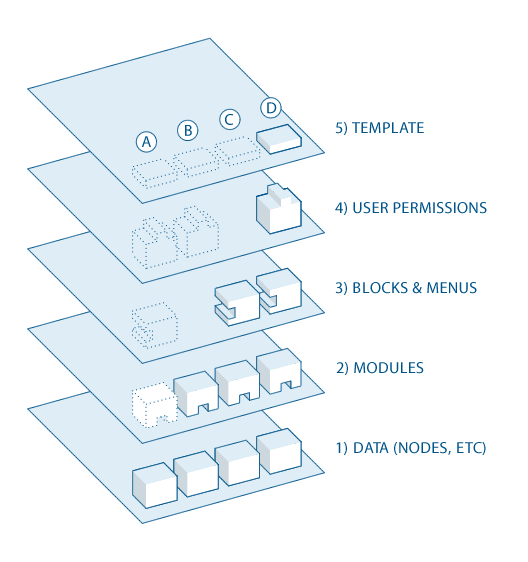
\includegraphics[width=14cm]{Chapter3/drupal_flow.png}
\caption{Drupal Flow}
\label{fig:drupal_flow}
\end{figure}

\begin{itemize}
\item At the base of the system is the collection of nodes—the data pool. Before anything can be displayed on the site, it must be an input as data.
\item The next layer up is where modules live. Modules are functional plugins that are either part of the Drupal core (they ship with Drupal) or they are contributed items that have been created by members of the Drupal community. Modules build on Drupal's core functionality, allowing you to customize the data items (fields) on your node types; set up e-commerce; programmatically sort and display content (custom output controlled by filters you define); and more. There are thousands of different options within the fast-growing repository of contributed Drupal modules. They represent the innovation and collaborative effort of everyone from individuals to large corporations.
\item At the next layer, we find blocks and menus. Blocks often provide the output from a module or can be created to display whatever you want, and then can be placed in various spots (Regions) in your template (theme) layout. Blocks can be configured to output in various ways, as well as only showing on certain defined pages, or only for certain defined users. Menus are navigators in Drupal, which define the content coming in each defined menu path. Menus are a core element of Drupal which provide links to all the pages created in Drupal.
\item Next are user permissions. This is where settings are configured to determine what different kinds of users are allowed to do and see. Permissions are defined for various roles, and in turn, users are assigned to these roles in order to grant them the defined permissions.
\item On the top layer is the site theme. This is made up predominantly of XHTML and CSS, with some Twig variables intermixed, so Drupal-generated content can go in the appropriate spots. Also included with each theme is a set of functions that can be used to override standard functions in the modules in order to provide complete control over how the modules generate their markup at output time. Templates can also be assigned on-the-fly based on user permissions.
\end{itemize}

This directional flow from bottom to top controls how Drupal works. Is some new functionality you want not showing up? Perhaps you uploaded the module into the system but have not activated it yet, and this is making everything downstream non-functional.

Maybe the module is installed and activated, but you still don’t see what you want on your site. Did you forget to place the block, as in "B"? Or are your user permission settings conflicting with what you want and your users are not set to see the output as in "C"?

Additionally as mentioned earlier getting the kind of granular control you want over the details of the XHTML module outputs requires understanding this flow. Are you using a module that does exactly what you want, only you wish the markup was just a little bit different? Maybe you’d like it to use different tags, or you’d like to assign a CSS class to something? You accomplish this by copying the output function from the module and pushing it up to the functions document in your theme. Modify the code there, and when the system goes to output, it will see your customized function and use that instead.

\subsection{Distribution}

mGov represents a Drupal distribution, which is a full copy of Drupal that include Drupal Core, along with additional software such as themes, modules, libraries, and installation profiles. There are two main types of Drupal distributions:

\begin{itemize}
	\item full-featured distributions: complete solutions for specialized use cases.
	\item other distributions: quick-start tools, starting points for developers and site builders.
\end{itemize}

\subsubsection{What is a distribution?}

Setting up a Drupal site typically involves downloading and configuring Drupal core, then downloading and configuring various contributed modules, as needed. To make this process easier, there are a variety of pre-configured versions of Drupal you can download and use for specific types of sites, for example a blogging site, a conference site, a corporate Intranet site, and so on. These 'pre-configured' versions of Drupal are called 'distributions'.

With a 'full-featured' distribution, you can quickly and easily set up a site for a specialized purpose, such as academic, business, government, nonprofit, publishing, social, in just a few steps:

\begin{itemize}
	\item choose your Drupal distribution.
	\item install it on your web server.
	\item configure it and enable the desired features from your website's Administer section.
\end{itemize}

\subsubsection{Distributions and installation profiles}

Installation profiles are what a developer creates as the basis of distributions. They define installation steps such as enabling modules, defining content types, etc.) that run after Drupal's base installation when you first install Drupal. One or more standard installation profiles are included in the Drupal Core download; developers can create custom profiles that set up Drupal for specific purposes, and optionally release them for community use on Drupal.org. It is not always easy to attempt to use an installation profile directly, if it requires non-core modules, themes, or libraries -- you would have to locate and download all the required components yourself before you could install Drupal. Instead, it's a lot easier to download a full distribution (if available).

Distributions are full copies of Drupal that include Drupal Core, along with additional software such as themes, modules, libraries, and installation profiles. The automatic packaging scripts on Drupal.org turn installation profiles into distributions, by gathering all the modules, themes, and libraries they require into a single zip archive, so that all you need to do is download the full archive and run the install script.

\subsubsection{When we need distributions?}

There are no hard and fast rules about when to use distributions, but here are a few guidelines:

\begin{itemize}
	\item evaluating Drupal: If you're just getting started with Drupal it makes sense to try a distribution, since they are easier to set up and you can see real-life examples of what Drupal can do. Not all distributions are equal though, so start with a popular well-maintained distribution.
	\item demoing Drupal: Before building a site for someone it can be useful to show them examples of how Drupal can be configured.
	\item quickly building a site: If you're building a site similar to one provided by a distribution it makes sense to start with a distribution. After installing you can continue to configure the site, add modules, create themes, etc. You can even undo things that the installation profile script may have done. If you're changing too much, though, it may make more sense to just start with stock Drupal and build from there, rather than try to undo and change what was set up for you.
	\item learning Drupal: In the administration section of a distribution, you can study the inner workings of a real example Drupal site, learn all the details about how it is built and configured to obtain specific functionality, and experiment with any changes and additional modules and themes.
\end{itemize}

\subsubsection{Creating Drupal Installation Profile}

Installation profiles in Drupal 8 have all the functionality of modules, including access to hooks and plugins and, critically, the ability to provide configuration for your site in the form of .yml files. First, you need a machine name for your profile. This is a name consisting of lowercase letters and underscores only, in our case is mgov\_kit.

Your installation profile will reside in its own profilename directory in the /profiles directory of a Drupal 8 site.
All installation profiles must have a profilename.info.yml file. They may also have:

\begin{itemize}
	\item profilename.profile
	\item profilename.install file
	\item config folder
	\item translations folder
\end{itemize}

When packaged, your installation profile will also have modules, src, and themes directories as needed.

The profilename.info.yml file should look similar to this:

\begin{lstlisting}[caption={.info.yml file},label={profile-file}]
name: Profile Name
type: profile
description: 'Description of your profile.'
core: 8.x

# Optional: Declare your installation profile as a distribution
# This will make the installer auto-select this installation profile.
# The distribution_name property is used in the installer and other places as
# a label for the software being installed.
distribution:
  name: Distribution Name
  # If you want your distribution to pre-select a language you can specify
  # the language code, as well. This will prevent the user from selecting
  # a language code in the user interface. While not recommended for generic
  # community distributions, this can be very useful for distributions that
  # are tailored to a language-specific audience (for example government
  # institutions in a certain country) but also site-specific installation
  # profiles. Note that this language code will also be used when installing
  # the site via Drush.
  langcode: de

# Required modules
dependencies:
  - node
  - history
  - block
  - block_content
  - breakpoint
  - color
  - config
  - comment
  - contextual
  - contact
  - quickedit
  - help
  - image
  - options
  - path
  - taxonomy
  - dblog
  - search
  - shortcut
  - toolbar
  - field_ui
  - file
  - rdf
  - views
  - views_ui
  - editor
  - ckeditor
\end{lstlisting}

\begin{lstlisting}[caption={.install.yml file},label={install-file}]
<?php
/**
 * @file
 * Install, update and uninstall functions for the profilename install profile.
 */

/**
 * Implements hook_install().
 *
 * Perform actions to set up the site for this profile.
 *
 * @see system_install()
 */
function profilename_install() {
  // First, do everything in standard profile.
  include_once DRUPAL_ROOT . '/core/profiles/standard/standard.install';
  standard_install();
  
  // Can add code in here to make nodes, terms, etc.
}
\end{lstlisting}

The profilename.profile file has access to almost everything a normal Drupal modulename.module file does because Drupal is fully bootstrapped before almost anything in the profile runs.

\begin{lstlisting}[caption={.profile.yml file},label={profile-file}]
<?php
/**
 * @file
 * Enables modules and site configuration for a standard site installation.
 */

// Add any custom code here like hook implementations.
\end{lstlisting}

Drupal 8 installation profiles can contain configuration files. You can start by taking the configuration directory (config folder) of an installed, configured site and copying it into the config/install folder in your profile.

Once that's in place, there are some other required tasks:

\begin{itemize}
	\item Copy all of the modules and themes listed within core.extension.yml into your profile's info file (using the new info file's format).
	\item Delete core.extension.yml (and possibly some other config files).
	\item Remove all of the UUIDs from your config files so that they don't conflict with those of new sites. This can be done quite easily on the command line like so all on one line:
\end{itemize}

\begin{lstlisting}[caption={.info.yml file},label={profile-file}]
find /path/to/PROFILE_NAME/config/install/ -type f -exec sed -i '' -e '/^uuid: /d' {} \;
\end{lstlisting}

If you just want to grab an existing site's configuration, and don't need to end up with a formal installation profile (for sharing on Drupal.org, for example), you can use the Configuration Installer installation profile to install a new site from the configuration of another site.

\subsection{Custom Modules}

Drupal 8 leverages a number of advanced PHP language features and sophisticated 3rd party libraries in order to present 3rd party developers with the most advanced API of any CMS available. While experienced Drupal 7 developers may see some significant changes, much of the basic structure will remain familiar.

If any of the material presented while going through the D8 module developer's walk-through is new to you, then the material below may help. However, a comprehensive knowledge is not necessary to proceed to the D8 module walkthrough.

\subsubsection{Object Oriented Programming}

OOP, while initially daunting, is now well established as a best practice.
For a general overview of PHP best practices, read through phptherightway.com. Drupal doesn't make use of all the different tools and techniques documented there but it does serve as a great introduction to PHP and the language's many features.

\subsubsection{Symfony 2}

Symfony 2 is a PHP framework that Drupal borrows from in order to reduce code duplication across various PHP projects. Much of the code that Drupal 8 uses to handle routing, sessions and the services container, amongst other things, is borrowed from Symfony 2.

A framework is not absolutely necessary: it is 'just' one of the tools that is available to help you develop better and faster!
Better, because a framework provides you with the certainty that you are developing an application that is in full compliance with the business rules, that is structured, and that is both maintainable and upgradable.
Faster, because it allows developers to save time by re-using generic modules in order to focus on other areas. Without, however, ever being tied to the framework itself.
A framework is not an absolute necessity, but nonetheless it is very useful. A framework is a pledge of quality, upgradability and maintainability of applications at lower cost. Applications developed using a framework are interoperable with market standards.

Besides a framework, there are other solutions that are available to develop both Web sites and Web applications: Content Management System and their supplemental modules, as well as packaged professional solutions. If their native features line up perfectly with your immediate and future needs, no question about it. There is no point in reinventing the wheel.



% realizarea sistemului, unde se explică cum a fost implementat sistemul, ce algoritmi și ce tehnologii au fost folosite ( se recomandă 20 pagini, include descrierea la nivel de cod);
